% !TEX root = ../foundations.tex

\section{Manifolds with corners}\label{S: manifolds with corners}

In this section, we provide an overview of manifolds with corners, which are the main geometric objects in the definitions of geometric chains and cochains.
Our reference for this material is Joyce \cite{Joy12}.
By \textbf{smooth} we always mean differentiable of all orders.
Throughout the paper, all manifolds and maps will be in the smooth category unless noted otherwise.

\begin{definition}
	If $A \subset \R^n$ and $B \subset \R^m$ are any subsets, we say that $f \colon A \to B$ is \textbf{smooth} if it extends to a smooth map from an open neighborhood of $A$ to $\R^m$.
	We say that $f$ is a \textbf{diffeomorphism} if $f$ is a homeomorphism and both $f$ and $f^{-1}$ are smooth\footnote{Joyce requires $n = m$ in his definition for $f$ to be a diffeomorphism.
	But suppose $f$ is a diffeomorphism as defined here and, without loss of generality, $n>m$.
	Let $\R^m \subset \R^n$ in the usual way.
	Then as $f$ extends to a smooth map from a neighborhood of $A$ to $\R^m$, we can certainly consider $f$ as extending to a smooth map from a neighborhood of $A$ to $\R^n$.
	Similarly, as $f^{-1}$ extends to a smooth map from a neighborhood of $B$ in $\R^m$ to $\R^n$, we can extend $f^{-1}$ to a neighborhood $B$ in $\R^n$ by precomposing with the projection $\R^n \to \R^m$.
	So diffeomorphisms in our sense can be made into diffeomorphisms in Joyce's sense, and obviously vice versa.}.
\end{definition}

With this definition, the notions of smooth charts and atlases for manifolds in the standard setting can be extended to define (smooth) manifolds with corners; see \cite[Section 2]{Joy12}: An $n$-dimensional chart $(U,\phi)$ of the space $W$ has domain $U$ an open subset of $\R^n_k = [0,\infty)^k \times \R^{n-k} \subset \R^n$, and $\phi$ is a homeomorphism from $U$ to $\phi(U) \subset W$.
Two $n$-dimensional charts $(U,\phi)$ and $(V,\psi)$ are compatible if $\psi^{-1}\phi \colon \phi^{-1}(\phi(U) \cap \psi(V)) \to \psi^{-1}(\phi(U) \cap \psi(V))$ is a diffeomorphism of subsets of $\R^n$.
An $n$-dimensional atlas for $W$ is a family of pairwise compatible $n$-dimensional charts that cover $W$, and an $n$-dimensional manifold with corners is a paracompact Hausdorff space with a maximal $n$-dimensional atlas.

While essentially equivalent, we choose to work entirely with subspaces of $\R^\infty$ in order to have a set of such objects, so rather than directly employ Joyce's definition, we define manifolds with corners for the purposes of this text as follows.

\begin{definition}\label{D: MWC}
	An $n$-dimensional \textbf{manifold with corners} $W$ is a subspace of some $\R^N \subset \R^\infty$ such that each point of $W$ possesses a neighborhood diffeomorphic to an open subset of $\R^n_k$ for some $k$.
\end{definition}

We note that these local diffeomorphisms provide charts $\phi \colon U \subset \R^n_k \to W$, and these charts are compatible, with $\psi^{-1}\phi \colon \phi^{-1}(\phi(U) \cap \psi(V)) \to \psi^{-1}(\phi(U) \cap \psi(V))$ being a diffeomorphism, even using Joyce's more restrictive notion of diffeomorphism.
These charts collectively give an atlas, and every atlas extends to a unique maximal one.
So our manifolds with corners are also manifolds with corners by Joyce's definition.

On the other hand, Joyce notes on page 231 of \cite{Joy12} that his manifolds with corners are what Melrose calls t-manifolds, and Melrose shows in \cite[Proposition 1.15.1]{Melrose} that t-manifolds can be embedded into manifolds without boundary.
These can then be embedded into Euclidean space by the Whitney Embedding Theorem.
So any one of Joyce's manifolds with corners is diffeomorphic to a manifold with corners in our sense.

By modeling on $\R^n_k$, our category includes manifolds ($k = 0$ in all charts) and manifolds with boundary ($k \leq 1$ in all charts), as well as cubes and simplices, but not the octahedron, for example, as the cone on $[0,1] \times [0,1]$ is not modeled by any $\R^n_k$.

\begin{comment}
	The smooth real-valued functions on a manifold with corners $W$ are those $f$ such that for each chart $\phi \colon U \subset \R^n_k \to W$ the composition $f \circ \phi \colon U \to \R$ is smooth.
\end{comment}

\begin{definition}
	A map $f \colon W \to M$ between manifolds with corners is {(weakly) \bf smooth} if whenever $(U,\phi)$, $(V,\psi)$ are charts for $W$ and $M$ respectively then
	$$\psi^{-1}f \phi \colon (f\phi)^{-1}\psi(V) \to V$$
	is smooth.

	The \textbf{tangent bundle} of a manifold with corners is the space of derivations of the ring of smooth real-valued functions.
	Analogously to smooth manifolds with boundary, if $(U,\phi)$ is a chart of $W$ then $d\phi$ takes the tangent space to $\R^n$ at $x \in U$ isomorphically to the tangent spaces of $W$ at $\phi(x)$.
	In particular, if $W$ is $n$-dimensional and $x \in W$, then the tangent space at $x$, denoted $T_xW$, is isomorphic to $\R^n$.
\end{definition}

In \cite{Joy12}, Joyce reserves the word \textit{smooth} for weakly smooth maps that also satisfy an additional condition concerning how they interact with the boundaries of their codomains.
When the codomain is a manifold without boundary, which will be our primary situation of interest, the weaker and stronger notions coincide.
In the few other cases in which we need to consider maps whose codomains have boundary, in particular boundary immersions and projections of pullbacks, the maps will also satisfy Joyce's stronger condition, though we will never need to utilize this explicitly.
Thus we will feel justified in simply using the word ``smooth'' throughout, referring the reader to \cite[Definition 3.1]{Joy12} for the full definition.

\begin{notation}
	Our default notation for manifolds with corners will be capital letters with the corresponding lower case letter denoting the dimension.
	In other words, $\dim(V) = v$, $\dim(W) = w$, $\dim(M) = m$, etc.
	We generally reserve $M$ for a manifold without boundary.
\end{notation}

\subsection{Boundaries}\label{S: boundaries}

We next need to describe boundaries of manifolds with corners.
Again see \cite[Section 2]{Joy12} for further details.

\begin{definition}
	A point $x$ in an $n$-dimensional manifold with corners $W$ has \textbf{depth} $k$ if there is a chart from an open subset of $\R^n_k$ which sends the origin to $x$.
	The set $S^k(W) \subseteq W$ of elements having depth~$k$ is called the \textbf{stratum of depth $k$}.
	By \cite[Proposition 2.4.]{Joy12}, $S^k(W)$ is an $n-k$ manifold without boundary.
\end{definition}

\begin{example}
	If $W$ is a smooth manifold with boundary in the classical sense, then $S^0(W)$ is its interior, $S^1(W)$ is its boundary, and $S^k(W) = \emptyset$ for $k>1$.
	If $S^k(W) = \emptyset$ for all $k>0$, then $W$ is a manifold without boundary.
\end{example}

When $W$ is a general manifold with corners, the boundary is more naturally a space equipped with a map to $W$, rather than a subspace of $W$.
The reason can be seen, for example, in the teardrop space of \cref{F: teardrop}, where the boundary should be considered to be homeomorphic to the closed interval mapping both endpoints to the vertex of the tear drop.
To explain in more detail, we have the following definitions.

\begin{figure}[h]
	\documentclass[tikz]{standalone}

\begin{document}
	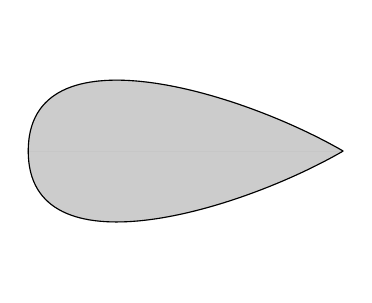
\begin{tikzpicture}[scale=4, rotate=90]
	\coordinate (a) at (0,1.2);
	\coordinate (b) at (0,0.2);

	\draw[out=120, in=180, fill, opacity=.2] (b) to (a);
	\draw[out=120, in=180] (b) to (a);
	\draw[out=60, in=0, fill, opacity=.2] (b) to (a);
	\draw[out=60, in=0] (b) to (a);
	\end{tikzpicture}
\end{document}
	\caption{The 2-dimensional ``teardrop'' is a manifold with corners whose boundary inclusion is not injective.}
	\label{F: teardrop}
\end{figure}

\begin{definition}
	A \textbf{local boundary component} $\beta$ of $W$ at $x \in W$ is a consistent choice of connected component $\mathbf{b}_V$ of $S^1(X) \cap V$ for any neighborhood $V$ of $x$, with consistent meaning that $\mathbf{b}_{V \cap V'} \subset \mathbf{b}_{V} \cap \mathbf{b}_{V'}$.
\end{definition}

Since this notion is local, the number of such components is determined by the depth.
Considering the origin in $\R^n_k$, for any $k \geq 0$, points having depth $k$ have exactly $k$ local boundary components.
As another example, letting $\interval = [0,1]$ and so $\interval^3$ the 3-cube, the set $S^1(\interval^3)$ consists of the interiors of two-dimensional faces, $S^3(\interval^3)$ is the set of eight corners, and any sufficiently small neighborhood of a corner intersects exactly three of the two-dimensional faces.

\begin{definition}\label{D: MWC boundary}
	Let $W$ be a manifold with corners.
	Define its \textbf{boundary} $\bd W$ to be the space of pairs $(x, \bb)$ with $x \in W$ and $\bb$ a local boundary component\footnote{Note that if $x \in S^0(W)$ then $x$ does not have any local boundary components and so does not appear in such a pair.} of $W$ at $x$.
	Define $i_{\bd W} \colon \bd W \to W$ by sending $(x,\bb)$ to $x$.
\end{definition}

In the teardrop example, $i_{\bd W} \colon \bd W \to W$ takes $\interval$ to the topological manifold boundary with both endpoints going to the unique point of $S^2(W)$.
For $\interval^3$, the boundary consists of six closed two-dimensional squares each mapping homeomorphically to a face of the cube.
In general, $|i_{\bd W}^{-1}(x)|$ is equal to the depth of $x$.

As in Douady \cite{Doua61}, $\bd W$ is itself a manifold with corners, and the boundary map $i_{\bd W}$ is a smooth immersion \cite[Theorem 3.4]{Joy12}. Note that $S^1(W)$ will always be diffeomorphic to the interior of $\bd W$, i.e.\ $S^0(\bd W) = S^1(W)$.
Inductively, we let $\bd^k W$ denote $\bd (\bd^{k-1} W)$ with $\bd^0 W = W$, and we let $i_{\bd^k W}$ denote the composite of the boundary maps sending $\bd^k W$ to $W$. The map $i_{\bd^k W}$ takes $S^a(\bd^k W)$ onto $S^{a+k}(W)$, but not, in general, injectively.

\begin{remark}\label{R: bd diff}
	If $f \colon V \to W$ is a diffeomorphism of manifolds with corners then it must, in particular, take components of $S^i(V)$ diffeomorphically onto corresponding components of $S^i(W)$, and, consequently, given a local boundary component $\mathbf{b}$ at a point $x \in V$, the map $f$ picks out a corresponding local boundary component, say $f_*(\mathbf{b})$ in $W$. We obtain a diffeomorphism $f_\bd \colon \bd V \to \bd W$ by $(x,\mathbf{b})\mapsto (f(x),f_*(\mathbf{b}))$ with $fi_{\bd V} = i_{\bd W} f_\bd$.
\end{remark}

While for manifolds with boundary $\bd^2 W$ is empty, for general manifolds with corners it will not be.
However, given a co-oriented map $W \to M$, $\bd^2 W$ does come equipped with a natural co-orientation reversing $\Z_2$ action.
This will be explained below and is a key component in showing that $\bd$ is suitable for defining boundary maps of geometric chain and cochain complexes.

N.B. When no confusion is likely to occur, we will sometimes abuse notation and use $\bd W$ also to refer to the image $i_{\bd W}(\bd W) \subset W$, which is the boundary of $W$ as a topological manifold in the usual sense.

The following is an example in which $\bd^2 W$ immerses into $W$ in an interesting way.

\begin{example}\label{boundary}
	Consider the quotient $Q$ of $S^n \times \R^2_2$ by the diagonal $C_2$ action, where $C_2$ (the group of order 2) acts antipodally on $S^n$ and acts by permuting the two coordinates
	of $\R^2_2$.
	The projection of $Q$ onto $S^n / C_2 = \R P^n$ defines a fiber bundle with fiber $\R^2_2$.
	Local coordinates can then be used to endow $Q$ with the structure of a manifolds with corners.

	The subspace $S^1(Q)$ is diffeomorphic to $S^n \times (0,\infty)$, and $S^2(Q)$ is diffeomorphic to $\R P^n$.
	The boundary $\bd Q$ is the quotient of $S^n \times \bd \R^2_2$ by $C_2$, which is diffeomorphic to
	$S^n \times [0,\infty)$.
	Thus $\bd^2 Q$ is $S^n$, which maps to $S^2(Q)$ by the standard quotient by antipodal action.
\end{example}

In general, Proposition~2.9 of \cite{Joy12} identifies $\bd^k W$ with the set of points $(x,\bb_1,\ldots,\bb_k)$ with $x \in W$ and the $\bb_i$ providing an ordered $k$-tuple of distinct local boundary components of $W$.

\begin{comment}
	% , whose $\bd^3$ is two copies of the symmetric group on three letters.
	% $\bd^1(T \times [0,1])$..., $\bd^2(T \times [0,1])$..., $\bd^3 (T \times [0,1])$...
\end{comment}

Special cases of manifolds with corners, including
manifolds with faces or manifolds with embedded corners \cite{Joy12}, steer clear of the interesting boundary phenomena of \cref{boundary}.
Although, a more restrictive notion should suffice for our application, Lipyanskiy develops geometric cohomology in the current generality, and we appreciate Joyce's careful treatment of transversality in this category, so we use their definitions.

We conclude this section by observing that the product $V \times W$ of two manifolds with corners is naturally a manifold with corners with, by \cite[Proposition 2.12]{Joy12},
$$\bd (V \times W) = (\bd V \times W) \sqcup (V \times \bd W).$$

\subsection{Transversality}

Transversality of smooth maps will play a key role, as this is the condition that assures that intersections or, more generally, pullbacks of manifolds (with corners) are also manifolds (with corners).
Recall that in the classical setting if $f \colon V \to M$ and $g \colon W \to M$ are smooth maps of manifolds without boundary then we say that $f$ and $g$ are \textbf{transverse} if whenever $f(x) = g(y) = z$ for some $x \in V$, $y \in W$, and $z \in M$ we have $Df(T_xV)+Dg(T_yW) = T_z M$.
We here discuss the extension of transversality to manifolds with corners, though only in the case where $M$ is without boundary.
More general versions of transversality can be found in \cite[Section 6]{Joy12}.

\begin{definition}{\cite[Special case of Definition 6.1]{Joy12}}
	Let $f \colon V \to M$ and $g \colon W \to M$ be smooth maps of manifolds with corners to a manifold without boundary.
	We say $f$ and $g$ are \textbf{transverse} if whenever $x \in S^j(X)$ and $y \in S^k(Y)$ with $f(x) = g(y) = z$ then $Df|_{S^j(V)}(T_xS^j(V))+Dg|_{S^k(W)}(T_yS^k(W)) = T_zM$.
\end{definition}

While this particular formulation of transversality is given in terms of the behavior of $f$ and $g$ on the strata $S^j(V)$ and $S^k(W)$, it is sometimes useful to have a reformulation in terms of the boundaries $\bd^j V$ and $\bd^kW$.
This is the content of \cref{L: simple trans} below.

To establish notation, let $f \colon V \to M$ and $g \colon W \to M$ be maps from manifolds with corners to a manifold without boundary.
We say that $f$ and $g$ are \textbf{plainly transverse} if they are transverse as maps of manifolds in the classical sense, without special consideration of strata or boundaries.
To be explicit in the case that $x \in V-S^0(V)$ or $y \in W-S^0(W)$ with $f(x) = g(y)$, let $(U_x,\phi_x)$ and $(U_y,\phi_y)$ be charts with $\phi_x(0) = x$ and $\phi_y(0) = y$.
By definition of smoothness, there exist neighborhoods $N_x$ and $N_y$ of $0$ in $\R^v$ and $\R^w$, respectively, so that $f\phi_x$ and $g\phi_y$ extend to smooth maps $\psi_x \colon N_x \to M$ and $\psi_y \colon N_y \to M$.
Then $f$ and $g$ are plainly transverse at $x$ and $y$ if $D\psi_x(T_0 \R^v)+D\psi_y(T_0\R^w) = T_{f(x)}M$.
This property is independent of the involved choices as $D\psi_x(T_0 \R^v)$ is the limit of $D\psi_x(T_{a} \R^v)$ for $a$ taken along any smooth path in $U_x$, and this does not depend on the choice of $N_x$ or $\psi_x$, and similarly for $\psi_y$.

\begin{lemma}\label{L: simple trans}
	Let $f \colon V \to M$ and $g \colon W \to M$ be maps from manifolds with corners to a manifold without boundary.
	Then $f$ and $g$ are transverse if and only if $fi_{\bd^j} \colon \bd^jV \to M$ and $gi_{\bd^k} \colon \bd^kW \to M$ are plainly transverse for all $j,k$.
\end{lemma}

Note that, a priori, the latter is a stronger condition as it imposes conditions not just on the interior of strata but on their closures.

\begin{proof}
	First suppose $fi_{\bd^j}$ and $gi_{\bd^k}$ are plainly transverse for all $j,k$.
	Suppose $x \in S^j(V)$ and $y \in S^k(W)$ for some fixed $j,k$ and $f(x) = g(y)$.
	The preimage of $x$ under $i_{\bd^j}$ consists of $j!$ points in $S^0(\bd^jV)$, and $i_{\bd^j}$ maps a neighborhood of each such preimage point diffeomorphically to a neighborhood of $x$ in $S^j(V)$, and similarly for $y$.
	Let $\psi_x$ be the inverse diffeomorphism from a neighborhood of $x$ in $S^j(V)$ to a neighborhood of one of the preimages.
	Then $f|_{S^j(V)} = fi_{\bd^j}\psi_x$ in a neighborhood of $x$, and similarly for $y$.
	Since $fi_{\bd^j}$ and $gi_{\bd^k}$ are plainly transverse, and $\psi_x$ and $\psi_y$ are diffeomorphisms, it follows that $f|_{S^j(V)}$ and $g|_{S^k(W)}$ are transverse at $f(x) = g(y)$.

	Conversely, suppose $f|_{S^j(V)}$ and $g|_{S^k(W)}$ are transverse for all $j,k$, and suppose $x \in \bd^jV$ and $y \in \bd^kW$ for some fixed $j,k$ with $fi_{\bd^j}(x) = gi_{\bd^k}(y) = z$.
	Furthermore, suppose $i_{\bd^j}(x) \in S^a(V)$ and $i_{\bd^k}(y) \in S^b(W)$, which implies $x \in S^{a-j}(\bd^j V)$.
	By focusing on local charts, there is a neighborhood of $x$ in $\bd^j(V)$ whose intersection with $S^{a-j}(\bd^j V)$ maps diffeomorphically via $i_{\bd^j}$ onto a neighborhood of $i_{\bd^j}(x)$ in $S^a(V)$, and analogously for $y$.
	Thus, $f|_{S^a(V)}i_{\bd^j}|_{S^{a-j}(\bd^j V)}$ and the analogous $g|_{S^b(W)}i_{\bd^k}|_{S^{b-k}(\bd^k W)}$ are transverse at $f(x) = g(y)$ as they precompose transverse maps with local diffeomorphisms.
	But the image of $D_x(fi_{\bd^j})$ contains the image of $D_x(f|_{S^j(V)}i_{\bd^j}|_{S^{a-j}(\bd^j V)})$ and similarly for $y$, and thus the images of $D_x(fi_{\bd^j})$ and $D_y(gi_{\bd^k})$ must also span $T_{z}M$.
	Therefore, $fi_{\bd^j}$ and $gi_{\bd^k}$ are plainly transverse at $f(x)$.
\end{proof}

\subsubsection{Achieving transversality}

Throughout this text, we will need a series of increasingly more general results guaranteeing that we can make certain maps transverse to each other.
We begin here with a relatively simple case that will be first used in \cref{S: basic properties} to show that geometric cohomology is contravariantly functorial with respect to continuous maps of manifolds without boundary.
All of our transversality theorems will be built using some basic tools that can be found in \cite[Section 2.3]{GuPo74}.
In particular, we record the following results, referring the reader to \cite[Section 2.3]{GuPo74} for the proofs\footnote{We rephrase the statements of these theorems slightly to better fit our context and notation.}:

\begin{theorem}[Transversality Theorem]
	Suppose $F \colon X \times S \to Y$ is a smooth map of manifolds, where only $X$ has boundary, and let $Z$ be any boundaryless submanifold of $Y$.
	If both $F$ and $F|_{\bd X \times S}$ are transverse to $X$, then for almost every $s \in S$, both $F(-,s) \colon X \to Y$ and $F(-,s)|_{\bd X} \colon \bd X \to Y$ are transverse to $Z$.
\end{theorem}

\begin{theorem}[$\epsilon$-Neighborhood Theorem]
	For a compact boundaryless manifold $Y$ in $\R^M$ and a positive number $\epsilon$, let $Y_\epsilon$ be the open set of points in $\R^M$ with distance less than $\epsilon$ from $Y$.
	If $\epsilon$ is sufficiently small, then each point $w \in Y_\epsilon$ possesses a unique closest point in $Y$, denoted $\pi(w)$.
	Moreover, the map $\pi \colon Y_\epsilon \to Y$ is a submersion.
	When $Y$ is not compact, there still exists a submersion $\pi \colon Y_\epsilon \to Y$ that is the identity on $Y$, but now $\epsilon$ must be allowed to be a smooth positive function on $Y$, and $Y_\epsilon$ is defined as $\{w \in \R^m \mid |w-y|<\epsilon(y) \text{\ for some\ } y \in Y\}$.
\end{theorem}

These theorems are used in \cite{GuPo74} to prove the following basic transversality result:

\begin{theorem}[Transversality Homotopy Theorem]
	For any smooth map $f \colon X \to Y$ and any boundaryless submanifold $Z$ of the boundaryless manifold $Y$, there exists a smooth map $g \colon X \to Y$ homotopic to $f$ such that $g$ is transverse to $Z$ and $g|_{\bd X}$ is transverse to $Z$.
\end{theorem}

Among other generalizations as we progress, we will extend these results to maps of manifolds with corners.
We will also often require that the homotopies take a special form, i.e.\ that they are \textit{universal} homotopies as defined in \cref{S: transverse cochains}.
See, for example, \cref{P: perturb transverse to map}.

The following technical lemma will help us extend the results of \cite{GuPo74} from transversality with respect to submanifolds to transversality with respect to maps.

\begin{lemma}\label{L: all transversality is wrt embeddings}
	Let $f \colon V \to M$ and $g \colon W \to M$ be smooth maps from manifolds with corners to a manifold without boundary.
	Let $e \colon W \to M \times \R^n$ be an embedding such that $\pi e = g$, where $\pi$ is the projection $M \times \R^n \to M$.
	Then $f$ and $g$ are transverse if and only if $e$ is transverse to $f \times \id_{\R^n} \colon V \times \R^n \to M \times \R^n$.
\end{lemma}

\begin{proof}
	It suffices to assume that $V$ and $W$ are without boundary.
	Otherwise we can apply the following argument to each pair of strata of $V$ and $W$.

	Suppose that $f$ and $g$ are transverse, i.e.\ that if $f(v) = g(w)$ then $Df(T_vV)+Dg(T_wW) = T_{f(v)}M$.
	For each $w \in W$, we can write $e(w) = (g(w),e_\R(w)) \in M \times \R^n$.
	Now suppose $w \in W$ and $(v,z) \in V \times \R^n$ such that $e(w) = (f \times \id_{\R^n})(v,z)$.
	Then we have $(g(w),e_\R(w)) = (f(v),z)$.
	The image of the derivative of $f \times \id_{\R^n}$ at such a point will span $Df(T_vV) \oplus T_z(\R^{n}) = Df(T_vV) \oplus \R^{n}$, while the derivative of $e$ will take $a \in T_w(W)$ to $Dg(a)+ De_{\R}(a)$.
	But the image of $D(f \times \id_{\R^n})$ already includes $0 \oplus \R^{n}$, so subtracting off the second summand, $D(f \times \id_{\R^{n}})(T_{(v,z)}(V \times \R^n))+De(T_wW)$ contains $Dg(a)$.
	It follows that $D(f \times \id_{\R^{n}})(T_{(v,z)}(V \times \R^n))+De(T_wW)$ contains $Df(T_vV) \oplus 0$, $Dg(T_wW) \oplus 0$, and $0 \oplus \R^n$.
	Since $f$ and $g$ are transverse and $D(f \times \id_{\R^{n}})(T_{(v,z)}(V \times \R^n))+De(T_wW)$ is a vector space, it therefore contains all of $T_{f(v)}M \oplus \R^n = T_{e(w)}(M \oplus \R^n)$.
	So $f \times \id_{\R^n}$ and $e$ are transverse.

	Next suppose $f \times \id_{\R^n}$ and $e$ are transverse and that $f(v) = g(w) \in M$.
	Suppose $e(w) = (g(w),z)$.
	Then $e(w) = (f \times \id_{\R^n})(v,z)$.
	So, by definition and assumption,
	\begin{equation}\label{E: Quillen transverse}
		D(f \times \id_{\R^{n}})(T_{(v,z)}(V \times \R^n))+De(T_wW) = T_{e(w)}(M \times \R^n) = T_{f(v)}M \oplus \R^n.
	\end{equation}
	As $\pi$ is a submersion, the image of this tangent space under $D\pi$ is all of $T_{f(v)}M$.
	But $(D\pi)(De) = D(\pi e) = Dg$, so $(D\pi \circ De)(T_wW) = Dg(T_wW)$.
	Furthermore, letting $\pi_V \colon V \times \R^n \to V$ be the projection, we have $(D\pi)(D(f \times \id_{\R^{n}})) = D(\pi(f \times \id_{\R^{n}})) = D(f\pi_V) = (Df)(D\pi_V)$, so, as $D\pi_V \colon T_{(v,z)}(V \times \R^n) \to T_vV$ is surjective, we have $(D\pi)(D(f \times \id_{\R^{n}}))(T_{(v,z)}(V \times \R^n)) = Df(T_vV)$.
	So applying $D\pi$ to equation \eqref{E: Quillen transverse}, we get $Df(T_vV)+Dg(T_wW) = T_{f(v)}M$, and $f$ is transverse to $g$.
\end{proof}

\begin{theorem}\label{T: basic trans}
	Let $f \colon M \to N$ be a continuous map from a manifold with (possibly empty) boundary to a manifold without boundary, and let $g \colon V \to N$ be a smooth map from a manifold with corners.
	Then there is a homotopy $h \colon M \times I \to N$ such that $h(-,0) = f$, and $h(-,1)$ is smooth and transverse to $g$.
	If $f|_{\bd M}$ is already smooth and transverse to $g$, then we can find such an $h$ with $h(-,1) = f$ on $\bd M$.
\end{theorem}

\begin{proof}
	Let $j \colon V \to \R^k$ be an embedding (we recall that such an embedding always exists by our definition of manifolds with corners).
	Then $e \colon V \to N \times \R^k$ given by $e(x) = (g(x),j(x))$ is an embedding that satisfies the hypotheses of \cref{L: all transversality is wrt embeddings}, so by that lemma it suffices to find a homotopy such that $h(-,0) = f$ and $h(-,1) \times \id_{\R^k} \colon M \times \R^k \to N \times \R^k$ is smooth and
	transverse to $e(V)$.

	We first find a homotopy from $f$ to a smooth map that agrees with $f$ on $\bd M$ if $f|_{\bd M}$ is already smooth.
	This can be done by the smooth approximation theorem; see \cite[Theorem III.2.5]{Kos93}.
	So we assume for the rest of the proof that this first homotopy has been completed and that $f$ is a smooth map.
	We will first construct our homotopy to achieve transversality without consideration of whether or not $f$ is already transverse to $g$ on $\bd M$, and then we show how to modify the construction for that case.

	We can think of $N$ as properly embedded in some $\R^K$ by the Whitney Embedding Theorem \cite[Section 1.8]{GuPo74}, and we let $N_\epsilon$ be an $\epsilon$ neighborhood of $N$ in $\R^K$ with submersion $\pi \colon N_\epsilon \to N$.
	Let $D$ be the open unit ball in $\R^K$.
	We define a composite map $H \colon M \times D \to \R^K \to N$ by
	$$H(x,s) = \pi(f(x)+ \epsilon(x)s).$$
	We have $H(x,0) = \pi(f(x)) = f(x)$, and, since $\epsilon(x)>0$ for all $x$, the map $(x,s) \to f(x)+ \epsilon(x)s$ is a submersion onto its image in $\R^K$.
	As $\pi$ is also a submersion, so is $H$, and then $H \times \id_{\R^k} \colon M \times D \times \R^k \to N \times \R^k$ is a submersion.
	In particular, $H \times \id_{\R^k}$ is transverse to $e(V)$ and to $e(S^i(V))$ for each stratum $S^i(V)$ of $W$.
	We can now apply the Transversality Theorem (though with the parameter space $D$ in a slightly nontraditional location in the ordering of factors) to obtain that $H(-,s) \times \id_{\R^k}$ is transverse to $e(V) \times \R^k$ for almost every $s \in D$.
	If $W$ is a stratum of $V$, then this statement also holds replacing $V$ with $W$.
	It also holds, for the same reasons, replacing $M$ with $\bd M$.
	Since $V$ has a finite number of strata and $M$ and $\bd M$ are only two space, and since the intersection of a finite number of dense subsets is dense, it holds for almost every $s \in D$, that both $H(-,s) \times \id_{\R^k}$ and its restriction to $\bd M \times \R^k$ are transverse to every stratum of $V$.
	Now let $s_0$ be one such $s$, and let $h \colon M \times I \to N$ be given by $h(x,t) = H(x,ts_0)$.
	Then $h(x,0) = H(x,0) = \pi(f(x)) = f(x)$.
	While $h(x,1) = H(-,s_0)$ has the desired properties by construction.

	If $f|_{\bd M}$ is already transverse to $g$, we modify the construction as follows: Let $\rho \colon M \to [0,1]$ be a smooth function that is $0$ on $\bd M$ and $>0$ on $M-\bd M$.
	Then we define
	$$H(x,s) = \pi(f(x)+ \epsilon(x)\rho(x)s).$$
	Then when $x \in \bd M$, we have $H(x,s) = \pi(f(x)) = f(x)$, so $h$ is constant along $\bd M$.
	For $x \notin \bd M$, the argument goes through exactly as above.
\end{proof}

\subsection{Pullbacks and fiber products}

When two embedded submanifolds of a manifold meet transversely, their intersection is again a submanifold.
More generally, if two smooth maps of manifolds are transverse, we can form their pullback, also called their fiber product, which is again a manifold.
This construction extends to manifolds with corners mapping into a manifold without boundary.

\begin{definition}\label{D: top pullback}
	Let $f \colon V \to M$ and $g \colon W \to M$ be transverse smooth maps from manifolds with corners to a manifold without boundary.
	Define the \textbf{pullback} or \textbf{fiber product} $V \times_M W$ by
	$$V \times _M W = \{(x, y) \in V \times W \mid f(x) = g(y)\}.$$

	There are canonical maps from $V \times _M W$ to $V$, $W$, and $M$ that respectively take $(x,y)$ to $x$, $y$, and $f(x) = g(y)$.
	\[
	\begin{tikzcd}
		V \times_M W \arrow[r, "g^*"] \arrow[d, "f^*"] & V \arrow[d, "f"] \\
		W \arrow[r, "g"] & M.
	\end{tikzcd}
	\]
	We typically suppress the maps from the notation, though we sometimes label them as in the diagram and sometimes write $f \times _M g \colon V \times _M W \to M$.
	We also sometimes write $f^*$ as $\pi_W$ and $g^*$ as $\pi_V$, as these maps are induced by restricting to $V \times _MW$ the projections from $V \times W$ to $V$ and $W$.

	We will generally use the term \textit{pullback} when we want to emphasize $V \times _M W$ with its map to $V$ or $W$, while the \textit{fiber product} is to be considered as mapping to $M$.
	When treating $V \times _M W$ as a pullback, we also sometimes use the notation $g^*V \to W$ or $f^*W \to V$; this notation is consistent with the analogous notation for pullbacks of fiber bundles, which is a special case.
\end{definition}

The following analysis of fiber products is standard -- see for example Proposition~7.2.7 of \cite{MaDo92}.

\begin{theorem}\label{pullback}
	Let $f \colon V \to M$ and $g \colon W \to M$ be transverse smooth maps from manifolds with corners to a manifold without boundary.
	Then $V \times _M W$ is a manifold with corners with
	\begin{equation*}
		S^i(V \times _M W) = \bigsqcup_{k + \ell = i} S^k(V) \times _M S^\ell(W).
	\end{equation*}
	Moreover, the maps from the fiber product to $V$, $W$, and $M$ are weakly smooth.
\end{theorem}

To generalize this theorem when $M$ is also a manifold with corners requires substantial additional hypotheses in the definition of transverse smooth maps.
Such a generalization is a central result in \cite{Joy12}.

There is a Leibniz rule for taking boundaries of fiber products of transverse maps \cite[Proposition~6.7]{Joy12}:
\begin{equation}\label{E: product boundary}
	\bd(V \times _M W) = (\bd V \times _M W) \sqcup (V \times _M \bd W),
\end{equation}
recalling that if $g \colon W \to M$ then we interpret $\bd W$ as equipped with the map $gi_{\bd W} \colon \bd W \to M$ and similarly for $V$.
We will see versions of this formula below that take into account orientations and co-orientations.

\subsubsection{Some further properties of transversality and fiber products}

In this section we collect some well known, though not always easy to find, results about transversality and fiber products.
We state these results mainly in the classical setting of manifolds without boundary, though they generally extend to the case of transverse maps of manifolds with corners mapping to a manifold without boundary, either by applying them to the pairwise transverse strata or by thinking in terms of ``plain transversality'' as defined above.

\begin{lemma}\label{L: tangent of pullbacks}
	Let $f \colon V \to M$ and $g \colon W \to M$ be transverse smooth maps of manifolds without boundary.
	Suppose $x \in V$ and $y \in W$ with $f(x) = g(y) = z$ so that $(x,y) \in V \times _MW$.
	Then the tangent space of $V \times _MW$ at $(x,y)$ as a subspace of $T_{(x,y)}(V \times W) = T_xV \oplus T_yW$ consists of those vectors $(\mathbf v,\mathbf w)$ such that $Df(\mathbf v) = Dg(\mathbf w) \in T_zM$.
	In other words,
	$$T_{(x,y)}(V \times _MW) = T_xV \times _{T_zM}T_yW,$$
	or ``the tangent space of the fiber product is the fiber product of the tangent spaces.''
\end{lemma}

A proof can be found in \cite[Theorem 5.47]{Wed16}.
Wedhorn proves this theorem for ``premanifolds,'' which are essentially manifolds minus the Hausdorff and second countability conditions.
These will be automatic in our setting, so Wedhorn's proof applies.
In many circumstances, this lemma allows us to reduce arguments about fiber products of maps of manifolds to arguments about fiber products of linear maps.

\begin{lemma}\label{L: normal pullback}
	Let $f \colon V \to M$ and $g \colon W \to M$ be transverse smooth maps of manifolds without boundary, and suppose $f$ is an embedding so that $V$ has a normal bundle $\nu V$ in $M$.
	Then the pullback map $g^*V = V \times _MW \to W$ is an embedding and the normal bundle of $g^*V$ in $W$ is isomorphic to the pullback of $\nu V$.
	In other words,
	$$g^*(\nu V) \cong \nu(g^*V).$$
	So ``the pullback of the normal bundle is the normal bundle of the pullback.''
	% anibal: in the previous lemma "or" was used instead of "So". Consider homogeneous style, maybe.

	In case $g$ is also an embedding, this allows us to identify the restriction of $\nu V$ to $V \cap W$ with a sub-bundle of $TW$ over $V \cap W$.
\end{lemma}

\begin{proof}
	See \cite[Proposition IV.1.4]{Kos93}.
\end{proof}

\begin{lemma}
	Let $f \colon V \to M$ and $g \colon W \to M$ be transverse smooth maps of manifolds without boundary, and suppose $f$ and $g$ are both embeddings.
	Then, identifying $V$ and $W$ as submanifolds of $M$, the fiber product $V \times _MW$ is simply the intersection $V \cap W$, which is a smooth submanifold of $M$.
\end{lemma}

\begin{proof}
	By \cref{L: normal pullback}, the pullback is a smooth submanifold of $W$, but $g$ is itself an embedding, so, identifying the manifolds with their embedded images, we obtain smooth submanifolds $V \times _MW \subset W \subset M$.
	That $V \times _MW = V \cap W$ in this situation follows immediately from the definition of the fiber product.
\end{proof}

The next lemma is a bit more specific but will be useful later in proving certain formulas.

\begin{lemma}\label{L: transverse to pullback}
	Let $f \colon V \to M$, $g \colon W \to M$, and $h \colon X \to W$ be smooth maps of manifolds without boundary, and suppose $f$ is transverse to $g$.
	Then $gh \colon X \to M$ is transverse to $f$ if and only $h$ is transverse to the pullback $\pi_W \colon g^*V \to W$.
\end{lemma}

\begin{proof}
	For simplicity of notation, let $P = g^*V = V \times _MW$, and let $\pi_V \colon P \to V$ and $\pi_W \colon P \to W$ be the maps induced by the projections from $V \times W$ to $V$ and $W$.
	So we have the diagram
	\[
	\begin{tikzcd}
		& P = V \times_M W \arrow[r, "\pi_V"] \arrow[d, "\pi_W"] & V \arrow[d, "f"] \\
		X \arrow[r, "h"] & W \arrow[r, "g"]&  M
	\end{tikzcd}
	\]
	First suppose $h$ is transverse to the pullback $g^*V \to W$.
	Note that the existence of $g^*V$ uses the assumption that $f$ and $g$ are transverse.
	Suppose $x \in X$ and $y \in V$ with $gh(x) = f(y)$.
	Then $(y,h(x)) \in P$, and by assumption we have both $Df(T_yV)+Dg(T_{h(x)}W) = T_{f(y)}M$ and
	$Dh(T_xX)+D\pi_W(T_{(y,h(x))}P) = T_{h(x)}W$.
	Applying $Dg$ to the second formula, we have
	$$Dg(T_{h(x)}W) = D(gh)(T_xX)+D(g\pi_W)(T_{(y,h(x))}P).$$
	So from the first formula,
	$$T_{f(y)}M = Df(T_yV)+D(gh)(T_xX)+D(g\pi_W)(T_{(y,h(x))}P).$$
	But $g\pi_W = f\pi_V$, so $D(g\pi_W)(T_{(y,h(x))}P) = D(f\pi_V)(T_{(y,h(x))}P) \subset Df(T_yV)$.
	It follows that
	$$T_{f(y)}M = Df(T_yV)+D(gh)(T_xX),$$
	i.e.\ $f$ is transverse to $gh$.

	Next suppose $f$ is transverse to $gh$ and that $x \in X, p \in P$ with $h(x) = \pi_W(p)$.
	As $gh(x) = g\pi_W(p) = f\pi_V(p)$, we have $gh(x)$ in the image of $f$, so in particular $gh(x)$ is in the intersection of the images of $V$ and $W$ in $M$.
	Now suppose $\mathbf w \in T_{h(x)}W$.
	By assumption $T_{hg(x)}M = Df(T_{\pi_V(p)}V)+D(gh)(T_xX)$, so we can write $Dg(\mathbf w) = Df(\mathbf a)+Dgh(\mathbf b)$ for some $\mathbf a \in T_{\pi_V(p)}V$ and $\mathbf b \in T_x X$.
	Now consider $\mathbf z = \mathbf w-Dh(\mathbf b) \in T_{h(x)}W$.
	Applying $Dg$ to both sides, we have $Dg(\mathbf z) = Dg(\mathbf w)-Dgh(\mathbf b) = Df(\mathbf a)$.
	So $(\mathbf a,\mathbf z)$ is in the pullback $T_{\pi_V(p)}V \times _{T_{gh(x)}M} T_{h(x)}W$.
	But by \cref{L: tangent of pullbacks}, this is precisely the tangent space of $V \times _MW$ at $(h(x),\pi_V(p))$.
	Furthermore, we have $D\pi_W(\mathbf a,\mathbf z) = \mathbf z$.
	Thus $\mathbf w = \mathbf z+Dh(\mathbf b) = D\pi_W(\mathbf a,\mathbf z)+Dh(\mathbf b)$.
	As $\mathbf w$ was arbitrary, $W = D\pi_W(T_{(h(x),\pi_V(p))}P)+Dh(T_xX)$, as desired.
\end{proof}

\subsubsection{Fiber products with more than two inputs}

Finally, we briefly consider transversality of more than two maps. Remark \ref{R: multiproducts} highlights some of the issues and difficulties involved, while Proposition \ref{P: 3 out of 4 trans} shows that there are still some simplifications that can be observed.

\begin{remark}\label{R: multiproducts}
	In this long remark we briefly discuss transversality and fiber products that involve more than two maps.
	This is relevant, for example, when considering associativity of fiber products or pullbacks of fiber products.
	As transversality of maps of manifolds is defined in terms of the behavior of the maps of tangent spaces, it is useful to first recall some notions about transversality in the setting of linear maps of vector spaces.

	If $f \colon V \to M$ and $g \colon W \to M$ are linear maps, then transversality of $f$ and $g$ can be expressed in a number of equivalent ways \cite[Section 4.7]{RamBas09}:
	\begin{itemize}
		\item $f(V)$ and $g(W)$ span $M$,
		\item the map $\Delta \colon V \times W \to M$ given by $\Delta(v,w) = f(v)-g(w)$ is surjective,
		\item $\dim(V \times _MW) = \dim(V)+\dim(W)-\dim(M)$.
	\end{itemize}
	The last two formulations easily generalize to $n$-tuples of maps $f_i \colon V_i \to M$.
	Such an $n$-tuple is considered transverse (as an $n$-tuple) when either of the following equivalent conditions hold:
	\begin{itemize}
		\item the map $\Delta \colon \prod V_i \to M^{n-1}$ given by $\Delta(v_1,\ldots,v_n) = (f_2(v_2)-f_1(v_1),\ldots, f_n(v_n)-f_{n-1}(v_{n-1}))$ is surjective,
		\item the fiber product given by $\{(v_1,\ldots,v_n) \in V_1 \times \cdots \times V_n \mid f_1(v_1) = \cdots = f_n(v_n)\}$ has dimension $\sum_{i = 1}^n\dim(V_i) -n\dim(M)$.
	\end{itemize}
	This version of transversality behaves very well in that this ``$n$-transversality'' is equivalent to the iterated transversality conditions that are required when taking fiber products two at a time.
	In other words, an $n$-tuple is transverse if and only if for any $1 \leq i<j \leq n$,
	\begin{itemize}
		\item the $j-i+1$-tuple $\{f_i,\ldots,f_j\}$ is transverse, and
		\item letting $P$ denote the fiber product of the maps $\{f_i,\ldots,f_j\}$, the $n-(j-i)$-tuple consisting of the fiber product map $P \to M$ and the $f_k$ with $k\notin\{i,\ldots,j\}$ is transverse.
	\end{itemize}
	Iterating this fact, we can see that this is equivalent to having $V_1$ transverse to $V_2$, then $V_3$ transverse to $V_1 \times _MV_2$ and so on.
	In particular, we can form the $n$-tuple fiber product if and only if we can form the \textit{transverse} iterated fiber products such as $(((V_1 \times _MV_2) \times _M V_3) \times _M\ldots) \times _M V_n$ as well as in any other order of association.
	See\footnote{Proposition 8-1 of \cite{RamBas09} actually concerns a more general situation of ``mixed associativity'' in which the data consists of zig-zags
	$$V_1 \xr{f_1}S_1\xl{g_2}V_1 \xr{f_2}\cdots \xr{f_{n-1}}S_{n-1}\xl{g_n}V_2.$$
	However, this reduces to our setting by taking $S_i = M$ and $g_i = f_i$ for all $i$.}
	\cite[Propositions~4-9 and 8-1]{RamBas09}.

	Unfortunately, in the setting of maps of manifolds (for the moment without corners), the situation is less well behaved.
	Let now $f_i \colon V_i \to M$ be an $n$-tuple of smooth maps of manifolds.
	We say that this $n$-tuple is transverse when for any $n$-tuple $(v_1,\ldots, v_n) \in V_1 \times \cdots \times V_n$ such that $f_1(v_1) = \cdots = f_n(v_n)$ the linear maps $D_{v_i}f_i$ are transverse.
	In this case, the fiber product $P = \{(v_1,\ldots, v_n) \in V_1 \times \cdots \times V_n \mid f_1(v_1) = \cdots = f_n(v_n)\}$ is a smooth manifold of dimension $\sum\dim(V_i)-(n-1)\dim(M)$.
	Furthermore, at any such point, this general transversality has implications such as those above for transversality of subcollections.

	However, the above relations between $n$-ary transversality and ``iterated transversality'' cannot hold in general, because the $n$-ary fiber product cannot necessarily know about all points in the iterated fiber product.
	For example, consider maps $f \colon V \to M$, $g \colon W \to M$, and $h \colon Z \to M$.
	Suppose that $f$ and $g$ are not transverse; in particular, we can suppose that the fiber product $V \times _MW$ is not a manifold.
	Further suppose that $h(Z)$ is disjoint from $f(V)$ and $g(W)$.
	In this case, the triple of maps is transverse (vacuously) and its 3-ary fiber product is well defined as $\emptyset$.
	However, the iterated fiber product $(V \times _MW) \times _M Z$ is not well defined in the category of smooth manifolds and maps.
	Given that we define fiber products only of transverse maps of smooth manifolds, in this case $V \times _M W$ is not properly defined in our category, and it is further impossible then to define $(V \times _MW) \times _M Z$ in this context.

	The upshot of all this is that when considering situations involving fiber products of more than two maps, we shall have to be careful about the transversality assumptions.
\end{remark}

Despite the preceding remark, the transversality conditions involved in associativity of fiber products are not completely independent, as the following proposition shows. In later sections, we will usually simply assume all needed transversality exists, but the following proposition can be useful in practice.

\begin{proposition}\label{P: 3 out of 4 trans}
	Let $f \colon V \to M$, $g \colon W \to M$, and $h \colon Z \to M$ be maps from manifolds with corners to a manifold without boundary. Suppose that $W$ is transverse to $Z$ and that $V$ is transverse to $W$ and to $W \times _MZ$. Then $V \times _MW$ is transverse to $Z$. In particular, if $V \times _M(W \times _MZ)$ and $V \times _MW$ are well defined, then so is $(V \times _MW) \times _M Z$.
\end{proposition}

\begin{proof}
	We must show that $V \times _MW$ is transverse to $Z$, so we consider points $(v,w) \in V \times _M W$ and $z \in Z$ such that $h(z)$ is equal to $(f \times _Mg)(v,w)$, which by definition is equal to $f(v) = g(w)$. In other words, we consider $(v,w,z) \in V \times W \times Z$ such that $f(v) = g(w) = h(z)$.

	So suppose $(v,w,z)$ is such a triple, and denote the common image by $m \in M$. By the transversality assumptions, we know that the images of $D_wg \colon T_wW \to T_mM$ and $D_z h \colon T_zZ \to T_mM$ span $T_mM$, i.e.\ that $D_wg$ and $D_zh$ are transverse as linear maps, and similarly that $D_{(w,z)}(g \times _M h) \colon T_{(w,z)}(W \times _M Z) \to T_mM$ is transverse to $D_vf \colon T_vV \to T_mM$. Furthermore, by Lemma \ref{L: tangent of pullbacks}, the tangent space of a fiber product is the fiber product of the tangent spaces, so $T_{(w,z)}(W \times _M Z) = T_wW \times _{T_mM}T_zZ$ and $D_{(w,z)}(g \times _M h) = D_wg \times _{T_mM}D_zh$.

	Now by \cite[Propositions~4-9]{RamBas09}, the triple of linear maps $(D_vf,D_wg,D_zh)$ is transverse as a triple of maps, if and only if both $D_wg$ is transverse to $D_zh$ and $D_wg \times _{T_mM}D_zh$ is transverse to $D_vf$. As such statements are independent of how we order the terms, the transversality established in the preceding paragraph also implies that $D_vf$ and $D_wg$ are transverse (which already follows from the hypotheses of the proposition), and $D_vf \times _{T_mM}D_wg$ is transverse to $D_zh$. But this implies, again using Lemma \ref{L: tangent of pullbacks}, that $h$ is transverse to $f \times _Mg$, as desired.
\end{proof}

\begin{remark}
	The end of the preceding proof at first seems to imply that if $g$ and $h$ are transverse and $g \times _M h$ is transverse to $f$, then $f$ is transverse to $g$ and $f \times _Mg$ is transverse to $h$. Indeed, \cite[Propositions~4-9]{RamBas09} says this is the case for the linear maps of the tangent spaces. Unfortunately, however, as \cite[Propositions~4-9]{RamBas09} applies only to linear maps, we can apply it only at those points $(v,w,z) \in V \times W \times Z$ where we know that $f(v) = g(w) = h(z)$ so that all three tangent space maps are well defined. So such a result would hold if the only intersections among the maps were such triple intersections. However, as noted in Remark \ref{R: multiproducts}, there could be pairs $(v,w) \in V \times W$ with $f(v) = g(w)$, but with this common image in $M$ not in the image of $h$. At such points, \cite[Propositions~4-9]{RamBas09} cannot tell us anything about the transversality of $V$ and $W$, and so $V \times _MW$ might not be well defined due to failure of transversality, even if $V \times _M (W \times _M Z)$ is.
\end{remark}